\documentclass[11pt,a4paper,twocolumn]{article}

% === Core Packages ===
\usepackage[margin=2cm]{geometry}
\usepackage[utf8]{inputenc}
\usepackage[T1]{fontenc}
\usepackage{times}
\usepackage{amsmath,amssymb}
\usepackage{graphicx}
\usepackage{booktabs}
\usepackage{float}
\usepackage{enumitem}
\usepackage{tikz}
\usepackage{pgfplots}
\pgfplotsset{compat=1.18}
\usetikzlibrary{arrows.meta,shapes.geometric,positioning,calc,decorations.markings,fit,backgrounds}

% === Citation (IEEE style) ===
\usepackage[numbers,sort&compress]{natbib}
\bibliographystyle{IEEEtranN}

% === Hyperref ===
\usepackage[hidelinks]{hyperref}
\usepackage{xurl}

% === Settings ===
\setlength{\parindent}{1em}
\setlength{\parskip}{0.3em}

% === PDF metadata ===
\hypersetup{
  pdftitle={Dreifstýrt orðsporsnet: Rammi fyrir náttúrulega samfélagsskipan},
  pdfauthor={Pavel Kudrna},
  pdfsubject={Personix — a decentralized reputation network},
  pdfkeywords={Personix, decentralized reputation, reputation social network,
    decentralized identifiers, DID, meritocracy, censorship resistance},
}

% === Title ===
\title{\textbf{Dreifstýrt orðsporsnet:\\Rammi fyrir náttúrulega samfélagsskipan}}
\author{Pavel Kudrna\\Personix Project --- \url{https://personix.org}\\Prague, Czechia\\Draft v1 --- March 2026}
\date{}

\begin{document}
\maketitle

% ============================================================
% ABSTRACT
% ============================================================
\begin{abstract}
Réttlætiskenndin---sannfæringin um að ranglæti verði leiðrétt og verðleikar verðlaunaðir---er sterkasti samloðunarkraftur samfélagsins. Þegar miðstýrðar stofnanir stjórnvalda geta ekki veitt þessa kennd vegna þess að kostnaðurinn við að framfylgja rétti er meiri en verðmæti réttarins sjálfs, veðrast samfélagsleg samloðun. Núverandi stofnanaskipulag nær ekki að leysa umtalsverðan flokk deilna á kerfisbundinn hátt, á sama hátt og miðstýrð áætlanagerð nær ekki að úthluta auðlindum: með ósamhverfum upplýsingum, brostnum endurgjafarrásum og því að ákvörðunartökuaðilar eru slitnir úr tengslum við afleiðingar ákvarðana sinna. Þessi grein kynnir orðspors-samfélagsnet (Reputation Social Network, RSN): dreifstýrt, óspillanlegt og ritskoðunarþolið samskiptalag byggt á dreifstýrðum auðkennum (Decentralized Identifiers, DID) sem gerir gerviauðkenndum þátttakendum kleift að birta, sannreyna og nýta orðsporsupplýsingar um hegðun í raunheimi. Kjarnaþátturinn hvílir á þremur hönnunarreglum: (1)~ósamhverfri kostnaðaruppbyggingu þar sem lestur orðsporsgagna er ódýr en ritun krefst sannreynanlegs erfiðis; (2)~óákvarðanlegri samskiptareglu um val sannreynenda byggðri á samræmdri tætingu (consistent hashing) sem verðleggur róttækar staðhæfingar með stigvaxandi ítrunarkostnaði; og (3)~markaðsdrifnu líkani orðsporsyfirvalds þar sem einkarekin sannreynendur veðja uppsöfnuðu orðspori sínu á nákvæmni þeirra staðhæfinga sem þeir styðja. Sú byggingarlist sem af þessu leiðir framleiðir verðleikaræði án miðstýrðrar samhæfingar og gerir kleift að fara smám saman og afturkræfa leið frá núverandi ríkisreknum kerfum.
\end{abstract}

% ============================================================
% 1. INTRODUCTION
% ============================================================
\section{Inngangur}

\subsection{Vandamál miðstýrðs trausts}

Nútíma stjórnun hvílir á grundvallarforsendu: að miðstýrðar stofnanir geti miðlað trausti milli ókunnugra í stórum stíl. Dómstólar dæma í deilum. Skrár votta eignarhald. Eftirlitsstofnanir framfylgja stöðlum. Þessar stofnanir voru hannaðar á tímum þegar upplýsingar voru af skornum skammti, samskipti hæg og valdaframsal til miðlægrar stofnunar eina raunhæfa samhæfingaraðferðin. Miðstýrð stjórnun bregst hins vegar af sömu byggingarlegu ástæðum og miðstýrð áætlanagerð: ósamhverfum upplýsingum, brostnum endurgjafarrásum og því að ákvörðunartökuaðilar eru slitnir úr tengslum við afleiðingar ákvarðana sinna.

Forsendan bregst til dæmis þegar kostnaðurinn við milligöngu stofnana er meiri en verðmæti deilunnar. Hugsum okkur leigjanda sem uppgötvar að leiguíbúð hans skortir lögbundið rafmagnsöryggisvottorð---ástand sem skapar bráða lífshættu. Lögbundinn réttur leigjandans til að segja sig frá samningnum er ótvíræður. Samt er kostnaðurinn við að framfylgja þeim rétti í gegnum dómskerfið meiri en fjárhagslegt verðmæti tryggingarinnar og skaðabótanna sem honum ber, jafnvel að meðtöldum hugsanlegum lögbundnum bótum~\cite{czcourtfees}. Skynsamlega svarið er að taka á sig tapið og hverfa á braut.

Þetta er ekki afbrigðilegt jaðartilfelli. Þetta er sjálfgefna upplifunin fyrir umtalsverðan flokk deilna þar sem skaðinn er raunverulegur en fjárhagslegu hagsmunirnir falla undir þröskuldinn þar sem framfylgd stofnana verður efnahagslega skynsamleg. Niðurstaðan er kerfi sem byggingarlega hyglir illa innrættum aðilum: þeir sem skaða aðra í magni undir þessum þröskuldi geta athafnað sig án afleiðinga, vegna þess að kostnaðurinn við að leita réttlætis fellur á þann sem skaðaður var.

Dæmið hér að ofan er sótt í lagaumhverfi höfundarins---tékkneska einkaréttarkerfið. Í öðrum réttarhefðum---fordæmisbyggðum almennum rétti (common law), venjurétti, blönduðum kerfum---bregst réttlætið á mismunandi hátt og í mismiklum mæli, allt eftir menningarlegum og málsmeðferðarlegum sérkennum lögsögunnar. Lesendur munu að öllum líkindum kannast við sambærileg dæmi úr eigin samhengi. Það sem er byggingarlega algilt er mynstrið: deilur þar sem verðmæti fellur undir þröskuld efnahagslega skynsamlegrar framfylgdar enda með því að sá sem skaðaður var tekur á sig tapið. RSN lofar ekki fullkomnu réttlæti---það dregur einfaldlega úr byggingarlega forskotinu sem illa innrættir aðilar njóta þegar framfylgd stofnana er óhagkvæm.

\subsection{Hvers vegna núverandi lausnir duga ekki}

\textbf{Rammar dreifstýrðra auðkenna (DID)}~\cite{did2022} veita dulkóðunaraðferðir fyrir sjálfstjórnandi auðkennisstýringu en einbeita sér fyrst og fremst að auðkennisstaðfestingu án þess að taka á víðtækari spurningunni um orðspor hegðunar.

\textbf{Sálbundnir tákn (Soulbound Tokens, SBT)}~\cite{weyl2022} fanga þá innsýn að orðspor sé óframseljanlegt en reiða sig á bálkakeðjuinnviði með skalanleikatakmörkunum og taka ekki á efnahagslegum hvötum sem stýra innskráningu upplýsinga. Skyld hugtök á borð við verðleikatákn (t.d. Liberland) deila svipaðri heimspeki en eru áfram bundin sérstökum lögsagnarrömmum.

\textbf{Dreifstýrð sjálfstæð samtök (Decentralized Autonomous Organizations, DAO)}~\cite{buterin2014} innleiða stjórnun með snjallsamningum en endurskapa auðræðislega hreyfiafla þar sem áhrif eru í hlutfalli við fjármagn. Ferningsleg atkvæðagreiðsla (quadratic voting)~\cite{buterin2019} dregur að hluta úr þessu en takmarkar hagnýta upptöku. DAO standa einnig frammi fyrir grundvallar\emph{véfréttarvandanum} (oracle problem): snjallsamningar geta ekki áreiðanlega sannreynt ástand í raunheimi án trausts ytri upprunaaðila, og þetta vandamál hefur enga almenna lausn innan byggingarlistar bálkakeðja.

Ekkert núverandi kerfi sameinar dreifstýringu, ritskoðunarþol, gervinafnleynd, sannreynanlegan aðgangskostnað og sjálfsprottna samstöðu.

\subsection{Framlög}

Þessi grein leggur fram eftirfarandi framlög:
\begin{enumerate}[nosep]
\item Skilgreiningu á \textbf{orðspors-samfélagsneti (RSN)}, dreifstýrðri samskiptareglu sem víkkar DID-rammann til að styðja tvíhliða orðsporsskipti.
\item \textbf{Óákvarðanlega samskiptareglu um val sannreynenda} byggða á samræmdri tætingu~\cite{karger1997}.
\item \textbf{Regluna um dýra róttækni} (Expensive Radicalism Principle), sem verðleggur staðhæfingar eftir fjarlægð þeirra frá samstöðu netsins um þrjár uppsafnaðar kostnaðarrásir.
\item \textbf{Líkan um orðsporshæft yfirvald} (Reputable Authority) með ósamhverfum hvötum þar sem fölsk stuðningsyfirlýsing kostar stórfellt meira en lögmæt gjöld.
\item \textbf{Leið smám saman umskipta} um samsíða skattkerfisinnviði.
\end{enumerate}

% ============================================================
% 2. DESIGN PRINCIPLES
% ============================================================
\section{Hönnunarreglur}

Byggingarlist RSN er bundin fimm ósemjanlegum hönnunarreglum.

\textbf{Samfella og þróun.} Kerfið lifir samhliða núverandi stofnunum á umskiptatímabili af óskilgreindri lengd. Umskiptin verða að vera afturkræf á hverju stigi.

\textbf{Sjálfviljugni og ábyrgð.} Þátttaka er sjálfviljug, en sjálfviljugni fylgir ábyrgð: þátttakandi sem tekur við stjórn stofnanahlutverks tekur um leið á sig meðfylgjandi skyldur.

\textbf{Fjölbreytni og menningarlegt hlutleysi.} Samstaða sprettur af tvíhliða samskiptum, ekki af fyrirframstilltum reglum sem kerfishönnuðir leggja á.

\textbf{Seigla og ritskoðunarþol.} Kostnaðurinn við að ritskoða netið verður að vera meiri en kostnaðurinn við að umbera það. Aðeins algjört alræði---með gríðarlegum pólitískum og efnahagslegum kostnaði---getur bælt kerfið niður.

\textbf{Samstaða og framfylgd.} Kerfið innlimar mannlega tilhneigingu til smásálar, hefndargirni og hefndarfullnægju sem burðarþætti. Misferli er ekki bannað; það er verðlagt.

% ============================================================
% 3. SYSTEM OVERVIEW
% ============================================================
\section{Yfirlit yfir kerfið}

\subsection{Orðspors-samfélagsnet}

RSN er dreifstýrt jafningjatengt samskiptalag þar sem þátttakendur skiptast á sannreynanlegum upplýsingum um hegðun í raunheimi. Skilgreinandi eiginleikar þess eru: dreifstýrður og óritskoðanlegur innviður; gervinafnleynd þátttöku í gegnum DID; ósamhverf kostnaðaruppbygging (lestur er ódýr, ritun er dýr); dulkóðunarleg sannreynanleiki; og \textbf{stuðningur við staðla}---vélalæsileg snið fyrir upplýsingar sem breiðast út um netið, fyrir þjónustu sem yfirvöld bjóða (samsetning staðhæfinga, stuðningsyfirlýsingar, vitnisþjónusta), og fyrir stefnusnið sem inniheldur reglur um mat á orðspori gagnaðila og mat á áhættu af misræmi stefnu (milli yfirlýstrar og raunverulegrar hegðunar).

\subsection{Byggingareiningar}

RSN samanstendur af fjórum meginþáttum (Mynd~\ref{fig:architecture}):
\begin{enumerate}[nosep]
\item \textbf{DID-lag.} Auðkenni þátttakenda með yfirlýstum reglum, orðsporslýsigögnum og netbeiningu.
\item \textbf{Staðhæfingarregla.} Skipulagt snið til að birta fullyrðingar um raunatburði.
\item \textbf{Sannreyningarnet.} Dreifstýrð samskiptaregla til að úthluta sannreynendum með samræmdri tætingu.
\item \textbf{Orðsporssamsöfnunarlag.} Þjónustur sem framleiða mannlæsileg orðsporsyfirlit.
\end{enumerate}

\begin{figure}[ht]
\centering
\begin{tikzpicture}[
    layer/.style={draw, minimum height=0.7cm, align=center, font=\scriptsize, fill=black!8},
    arr/.style={<->, thick, gray!60}
]
\node[layer, minimum width=5cm] (agg) at (0,2.8) {\textbf{Samsöfnun}\\Túlkun\ $\cdot$ Áhætta};
\node[layer, minimum width=2.2cm] (claim) at (-1.55,1.4) {\textbf{Staðhæfingar}\\Semja};
\node[layer, minimum width=2.2cm] (verif) at (1.55,1.4) {\textbf{Sannreyning}\\Val};
\node[layer, minimum width=5cm] (did) at (0,0) {\textbf{DID-lag}\\Auðkenni $\cdot$ Reglur $\cdot$ Einkunnir};

\draw[arr] (agg.south west) -- (claim.north);
\draw[arr] (agg.south east) -- (verif.north);
\draw[arr] (claim.east) -- (verif.west);
\draw[arr] (claim.south) -- (did.north west);
\draw[arr] (verif.south) -- (did.north east);
\end{tikzpicture}
\caption{Fjögurra laga byggingarlist RSN.}
\label{fig:architecture}
\end{figure}

\subsection{Hlutverk þátttakenda}

Sannreyningarviðskipti fela í sér allt að sex aðgreind DID-hlutverk (Mynd~\ref{fig:roles}): \textbf{Útgefanda} ($DID_I$, býr til og leggur fram staðhæfinguna), \textbf{Viðfang} ($DID_S$, það DID sem staðhæfingin fjallar um---getur farið saman við Útgefanda), \textbf{Yfirvald} ($DID_A$, styður staðhæfinguna gegn gjaldi; getur einnig boðið vitnisþjónustu---\emph{valfrjálst}), \textbf{Vitni} ($DID_{W_{1..n}}$, huliðsmeðvituð eftirlit með heiðarleika sannreynanda um áskorunarkóða---\emph{valfrjálst}), \textbf{Sannreynanda} ($DID_V$, valinn með reikniriti til að birta staðhæfinguna), og \textbf{RSN} (netið þar sem sannreyndar staðhæfingar eru birtar). Hvaða hlutverk sem er má framselja til annars DID (Kafli~7.4). Yfirvald tengir oft saman stuðningsyfirlýsingu og vitnisþjónustu, en hlutverkin tvö eru rökrænt óháð.

\begin{figure}[ht]
\centering
\begin{tikzpicture}[
    role/.style={draw, rounded corners, minimum width=1.1cm, minimum height=0.45cm, align=center, font=\scriptsize, fill=black!8},
    opt/.style={draw, rounded corners, minimum width=1.1cm, minimum height=0.45cm, align=center, font=\scriptsize, fill=black!8, dashed},
    arr/.style={-{Stealth[length=3pt]}, thick},
    oarr/.style={-{Stealth[length=3pt]}, thick, dashed, gray},
    lbl/.style={font=\tiny, fill=white, inner sep=1pt}
]
\node[role] (I) at (0,2.4) {\textbf{Útgefandi}};
\node[role] (S) at (-2.5,2.4) {\textbf{Viðfang}};
\node[opt] (A) at (2.5,1.2) {\textbf{Yfirvald}};
\node[opt] (W) at (-2.5,0) {\textbf{Vitni}};
\node[role] (V) at (2.5,-0.6) {\textbf{Sannreynandi}};
\node[role, fill=black!5, draw=gray] (N) at (0,-1.8) {RSN};

\draw[arr] (I) -- node[lbl] {um} (S);
\draw[oarr] (I) -- node[lbl,sloped] {styður} (A);
\draw[oarr] (I) -- node[lbl,sloped] {áskorun} (W);
\draw[arr] (I) -- node[lbl,sloped] {beiðni} (V);
\draw[oarr] (W) -- node[lbl] {fylgist með} (V);
\draw[arr] (V) -- node[lbl] {birtir} (N);
\end{tikzpicture}
\caption{DID-hlutverk í sannreyningarviðskiptum. Punktalínur = valfrjálst (Yfirvald, Vitni).}
\label{fig:roles}
\end{figure}

\subsection{Óspillanleiki: fjórir kraftar}

Óspillanleiki RSN sprettur ekki af einum þætti heldur af fjórum samhliða kröftum. Enginn er nægilegur einn og sér; aðeins samsetning þeirra gerir tilraun til spillingar efnahagslega óskynsamlega.

\textbf{Ófyrirsjáanlegt skotmark.} Sannreynandinn fyrir hverja staðhæfingu er valinn óákvarðanlega með samræmdri tætingu (Kafli~5.3). Árásaraðili getur ekki fyrirfram beint mútum að tilteknum sannreynanda, vegna þess að auðkenni sannreynandans er fall af efni staðhæfingarinnar og fyrri ítrunum, ekki af vali útgefandans.

\textbf{Orðsporsvogarafl---hægt upp, hratt niður.} Orðspor er aðeins hægt að ávinna smám saman, með viðvarandi samkvæmri hegðun. Það getur hins vegar glatast stórfellt í einni svikafullri stuðningsyfirlýsingu (Kafli~6.2). Þessi ósamhverfa þýðir að ára uppsafnaðs orðspors má eyðileggja með einni óheiðarlegri stuðningsyfirlýsingu; ákjósanlegasta stefnan er áfram að hafna grunsamlegum staðhæfingum.

\textbf{Opinbert loforð.} Sérhver DID-handhafi lýsir opinberlega yfir stefnu sinni---vélalæsilegu setti reglna sem hann skuldbindur sig til að fylgja. Frávik milli yfirlýsingar og raunverulegrar hegðunar er greinanlegt og verðlagt sem orðsporsbrot alvarlegra en undirliggjandi brotið sjálft (Kafli~7.3). Hræsni er því dýrari en bein óheiðarleiki.

\textbf{Ósamhverfa árásarkostnaðar í möskva.} Kostnaðurinn við að ritskoða eða koma netinu úr jafnvægi vex ólínulega með stærð og þéttleika netsins, á meðan kostnaðurinn við að umbera það helst óbreyttur. Til að ritskoðun borgi sig þyrfti miðstýrður aðili að beita henni um allt netið---sem krefðist aðgerða úr öllu hófi við hvaða hugsanlegan ávinning sem er (Kafli~10).

% ============================================================
% 4. DECENTRALIZED IDENTITY MODEL
% ============================================================
\section{Líkan dreifstýrðs auðkennis}

\subsection{DID með sérstökum eiginleikum}

RSN víkkar W3C DID Core forskriftina~\cite{did2022} með: \textbf{Yfirlýstum reglum} (vélalæsilegum hegðunarskuldbindingum), \textbf{Orðsporslýsigögnum} (samsafnaðri hegðunareinkunn), og \textbf{Netbeiningu} (breytanlegri laukhlið aðgreindri frá stöðugri hringstöðu).

\subsection{Líftími staðhæfingar}

Staðhæfing fer í gegnum sex stig (Mynd~\ref{fig:lifecycle}): samsetningu, valfrjálsa stuðningsyfirlýsingu yfirvalds, val sannreynanda með samræmdri tætingu, sannreyningarákvörðun (samþykki eða höfnun með ítrun), birtingu, og orðsporsuppfærslu fyrir alla aðila.

\begin{figure}[ht]
\centering
\begin{tikzpicture}[
    stp/.style={draw, rounded corners=2pt, minimum width=1.3cm, minimum height=0.45cm, align=center, font=\tiny, fill=black!5},
    arr/.style={-{Stealth[length=3pt]}, thick},
    lbl/.style={font=\tiny, fill=white, inner sep=1pt}
]
\node[stp] (comp) at (0,0) {Semja\\staðhæfingu};
\node[stp, dashed] (auth) at (2.0,0) {Yfirvald\\styður};
\node[stp] (hash) at (4.0,0) {Tæta og\\varpa á hring};
\node[stp] (ver) at (2.0,-1.6) {Sannreynandi\\athugar};
\node[stp, double] (pub) at (0,-1.6) {Birt};
\node[stp] (rej) at (4.0,-1.6) {Hafnað\\kostn. $\uparrow$};

\draw[arr] (comp) -- (auth);
\draw[arr] (auth) -- (hash);
\draw[arr] (hash) -- (ver);
\draw[arr] (ver) -- node[lbl] {\checkmark} (pub);
\draw[arr] (ver) -- node[lbl] {$\times$} (rej);
\draw[arr] (rej) -- ++(0,0.8) -| (hash);
\end{tikzpicture}
\caption{Líftími staðhæfingar með ítrunarlykkju.}
\label{fig:lifecycle}
\end{figure}

\subsection{Tengsl við W3C DID Core}

Auðkennislíkan RSN er eiginlegt yfirmengi W3C DID Core forskriftarinnar~\cite{did2022}. Öll RSN-DID eru gild W3C-DID. RSN-sértæku útvíkkanirnar eru kóðaðar sem eiginleikar DID-skjals sem skilgreindir eru í sérstakri forskrift DID-aðferðar, samhæfðri núverandi innviðum á borð við ION~\cite{buchner2021} og Ceramic~\cite{ceramic2023}.

% ============================================================
% 5. VERIFICATION AND PROPAGATION
% ============================================================
\section{Sannreyning og útbreiðsla upplýsinga}

\subsection{Kostnaður við innskráningu upplýsinga}

Kjarnahagfræðiregla RSN er ósamhverfan milli lesturs og ritunar. Lestur orðsporsgagna nálgast núll jaðarkostnað fyrir þátttakendur sem eru hluti af DID-netinu og hafa aðgang í samræmi við orðspor sitt---nýliðar verða smám saman að ávinna sér víðtækari aðgang (sjá sníkjuvörn). Ritun---skilin sem varanleg efnisleg birting orðspors inn í netið, ekki sem einstakur tæknilegur verknaður---krefst sannreynanlegrar uppsafnaðrar fjárfestingar í þremur víddum: \textbf{tíma} (æviárum varið í samkvæma hegðun, uppfylltar skuldbindingar og ræktuð tengsl), \textbf{orku} (erfiði lagðu í heiðarleg viðskipti, umhyggju fyrir samstarfi og langtímaáreiðanleika), og \textbf{peningum} (fjárfestingu í eigin nafni---starfsþróun, gæðum eigin verka, endurgreiðslu fyrir valdinn skaða). Orðspor er ekki hægt að kaupa samstundis---það er afrakstur ævilangrar uppsöfnunar sem kerfið gerir einungis sýnilega og framseljanlega milli samhengja. Einstakur tæknilegur kostnaður samskiptareglunnar (dulkóðunarundirskriftir, gjöld sannreynenda) er hverfandi samanborið við þessa undirliggjandi fjárfestingu.

\subsection{Samfélagsgraf og tengsladýpt}

RSN er í grunninn samfélagsnet: hvert DID bætir við tengiliðum (öðrum DID) sem leyfa tenginguna. Þessir tengiliðir hafa sína eigin tengiliði, og svo framvegis. Reikniritsleg leit að sannreynanda starfar innan stillanlegrar dýptar $h$ tengdra tengiliða (t.d. $h=3$: eigin beinir tengiliðir, tengiliðir þeirra, og tengiliðir tengiliða). Þessi byggingarlist krefst ekki einnar altækrar bálkakeðju---hún hyglir eðlilega tilkomu samfélaga/klasa með skörun inn í önnur samfélög. Sérhver DID-þátttakandi verður að hafa birta \textbf{stefnu}---vélalæsilegt sett reglna sem stýrir því hvernig innkomnar beiðnir eru metnar. Stefnubrot eru skráð í netið sem neikvæðir gripir.

\subsection{Reikniritslegt val sannreynanda}

Sannreyningarreglan notar samræmda tætingu~\cite{karger1997} (Mynd~\ref{fig:verifier}). Sannreyning er gjaldskyld þjónusta: sannreynendur starfa gegn gjaldi og skapa markað þar sem samkeppni knýr verðlagningu, hraða og áreiðanleika.

\textbf{Skref 1.} Staðhæfingarskjalinu er skeytt saman við tætingarniðurstöðu fyrri ítrunar (eða $\varnothing$ í fyrstu ítrun) og það tætt:
\begin{equation}
\text{staða} = f_h(\text{staðhæfing} \| \text{fyrri\_tæting})
\label{eq:hash}
\end{equation}

Reikniritið verður að innihalda \emph{alla slóðina} allra fyrri beiðna og svara---ekki einungis tætingu fyrri ítrunar. Fullt svar hvers sannreynanda (samþykki, höfnun, uppgefið verð, ástæða) er bætt við vaxandi skjalið, sannreynanlegt með dulkóðunarundirskriftum við hvert skref.

\textbf{Skref 2.} Tætingunni er varpað á $N$ stöður á samræmda tætingarhringnum, jafndreift (t.d. fyrir $N=4$: $+0^{\circ}, +90^{\circ}, +180^{\circ}, +270^{\circ}$). Frá hverri stöðu velur réttsælis leit næsta DID sem sannreynandaframbjóðanda (Mynd~\ref{fig:multipoint}). $N$ er breytilegur breytustærð sem getur verið háð hlutfalli DID sem eru virk hverju sinni, tíma dags, eða sögulegri svörun netsins.

\textbf{Skref 3.} Sannreynandinn samþykkir (birtir og veðjar orðspori) eða hafnar (og snýr aftur á Skref~1 með höfnunartætingunni). Þegar hnútur svarar ekki þrátt fyrir yfirlýsta nettengingu verður næsta beiðni að innihalda öll svör frá öllum $N$ fyrri sannreynandaframbjóðendum.

\textbf{Sníkjuvörn.} Skotmarks-DID mega setja gjöld eða aðgangstakmarkanir á fyrirspurnir frá nýjum DID með lítið orðspor. Þetta stigskipta fyrirkomulag (ekki tvíundarlegt) þvingar nýliða til að byggja upp orðspor með raunverulegri virkni áður en þeir nýta frjálst gögn annarra.

\begin{figure}[ht]
\centering
\begin{tikzpicture}[
    box/.style={draw, rounded corners=2pt, minimum width=1.3cm, minimum height=0.45cm, align=center, font=\scriptsize, fill=black!5},
    dec/.style={draw, diamond, aspect=2.2, minimum width=0.9cm, align=center, font=\scriptsize, fill=black!5},
    arr/.style={-{Stealth[length=3pt]}, thick},
    lbl/.style={font=\tiny, fill=white, inner sep=1pt}
]
\node[box] (iss) at (0,0) {Útgefandi};
\node[box] (hash) at (0,-1.1) {$f_h$(staðhæf. $\|$\\fyrri\_tæting)};
\node[box] (ring) at (0,-2.2) {Hringvörpun\\réttsælis};
\node[box, dashed] (spam) at (0,-3.2) {Ruslpóstvörn\\innborgun};
\node[dec] (check) at (0,-4.4) {Stefnu-\\athugun};
\node[box] (rej) at (2,-5.6) {Næsta\\ítrun};
\node[box] (fee) at (0,-5.6) {Lokagjald =\\$f$(gögn, orðspor, stefna)};
\node[box, double] (pub) at (0,-6.8) {Birt};

\draw[arr] (iss) -- (hash);
\draw[arr] (hash) -- (ring);
\draw[arr] (ring) -- (spam);
\draw[arr] (spam) -- (check);
\draw[arr] (check) -- node[lbl] {$\times$} (rej);
\draw[arr] (check) -- node[lbl] {\checkmark} (fee);
\draw[arr] (fee) -- (pub);
\draw[arr] (rej.east) -- ++(0.5,0) |- (hash.east);
\end{tikzpicture}
\caption{Samskiptaregla um val sannreynanda. Ruslpóstvarnarinnborgun er valfrjáls og getur verið endurgreiðanleg. Lokagjald er aðeins greitt við samþykki.}
\label{fig:verifier}
\end{figure}

Hver höfnun bætir fullu svari sannreynandans (þar með talið ástæðum og skilyrðum) við staðhæfingarskjalið og víkkar efni þess. Frá víkkaða skjalinu er ný tæting reiknuð óákvarðanlega, sem varpast á aðra hringstöðu og velur annan sannreynanda. Skráning fullrar slóðar er skylda---útgefandinn getur ekki spáð fyrir um eða haft áhrif á næsta sannreynanda. Ef sannreynandi hunsar beiðni þrátt fyrir samhæfa yfirlýsta stefnu, skrá vitni (ef til staðar) það, og útgefandinn má hengja vitnaframburð við lokabirtingu.

\begin{figure}[ht]
\centering
\begin{tikzpicture}[scale=0.65]
% Ring
\draw[thick] (0,0) circle (2.2cm);
% DID nodes on ring
\foreach \a in {10,55,80,120,150,195,230,260,305,340} {
  \fill[black!40] (\a:2.2) circle (1.5pt);
}
% Hash offset arrow pointing to initial position
\draw[-{Stealth[length=3pt]}, thick, black!60] (0,0) -- node[font=\tiny,above,sloped,pos=0.6] {$f_h$} (37:2.2);
\fill[black] (37:2.2) circle (2pt);
\node[font=\tiny,anchor=south west] at (37:2.35) {$h_0$};
% N=4 points offset from h0 by +0, +90, +180, +270
\foreach \offset/\l in {0/P1,90/P2,180/P3,270/P4} {
  \pgfmathsetmacro{\ang}{37+\offset}
  \node[fill=black, circle, inner sep=1.5pt] (p\offset) at (\ang:2.2) {};
  \node[font=\tiny,font=\bfseries] at (\ang:2.75) {\l};
  % clockwise search arc
  \draw[-{Stealth[length=2.5pt]}, thick, gray] (\ang:2.2) arc (\ang:\ang+30:2.2);
}
\node[font=\scriptsize, align=center] at (0,0) {Tætingar-\\hringur};
\node[font=\tiny, align=center] at (0,-3.2) {$h_0 = f_h(\text{staðhæfing})$, síðan $+0^{\circ},+90^{\circ},+180^{\circ},+270^{\circ}$\\Hver punktur $\rightarrow$ réttsælis leit};
\end{tikzpicture}
\caption{Val með mörgum punktum ($N{=}4$). Tæting $h_0$ setur hliðrunina; 4 punktar jafndreifðir frá $h_0$.}
\label{fig:multipoint}
\end{figure}

\subsection{Vitnisregla}

\textbf{Vitnis}hlutverkið veitir huliðsábyrgð fyrir heiðarleika sannreynanda um dulkóðunarreglu áskorunarkóða:

\textbf{Skref V1.} Beiðandinn undirritar sannreyningarbeiðnina og sendir hana til $N_w$ vitna---tengiliða úr samfélagsneti beiðandans, eða sérhæfðra vitnisþjónustuveitenda sem starfa gegn gjaldi.

\textbf{Skref V2.} Hvert vitni $w_i$ undirritar alla undirrituðu beiðnina, heldur upprunalegu undirskriftinni $\sigma_i$, og reiknar áskorunarkóða $c_i = h(\sigma_i)$. Áskorunarkóðanum er bætt við beiðnina.

\textbf{Skref V3.} Beiðnin, sem nú ber $N_w$ áskorunarkóða, er send til sannreynandans. Sannreynandinn sér kóðana en \emph{getur ekki ákvarðað} hverjir vitnin eru eða hvort kóðarnir samsvara raunverulegum undirskriftum.

\textbf{Skref V4 (heiðarlegur sannreynandi).} Ef sannreynandinn svarar í samræmi við yfirlýsta stefnu sína, halda áskorunarkóðarnir ógagnsæi sínu. Vitnin eru aldrei afhjúpuð. Engin viðbótargögn eru birt.

\textbf{Skref V5 (stefnubrot).} Ef sannreynandinn brýtur gegn stefnu sinni (hunsar beiðnina, svarar ósamkvæmt), heldur beiðandinn upprunalegum undirskriftum vitnanna $\sigma_i$. Þessar má birta sem fylgigögn: hver sem er getur sannreynt $c_i = h(\sigma_i)$, sem sannar að vitnið var viðstatt. Beiðandinn getur birt sjálfstætt---sannreynandinn undirritaði þegar áskorunarkóðana í svari sínu.

\textbf{Blekkingareiginleikinn.} Beiðandinn má skipta út handahófskenndum gildum fyrir suma eða alla áskorunarkóða. Sannreynandinn getur ekki greint ekta kóða (studda af háorðspora yfirvöldum) frá suði. Þessi \emph{óvissa} er framfylgdarþátturinn: sérhver beiðni ber áhættuna á að virt yfirvald sé að fylgjast með huliðs. Kostnaðurinn við að viðhalda þessum þrýstingi er nálægt núlli (að framleiða handahófstölur), á meðan hugsanlegur kostnaður óheiðarleika fyrir sannreynandann er stórfelldur. Heiðarleg hegðun er hvött jafnvel í fjarveru raunverulegra vitna.

\textbf{Yfirvald sem vitni.} Yfirvald sem styður staðhæfingu má tengja við vitnisþjónustu: ,,Ég styð staðhæfingu þína og þjóna sem huliðsvitni meðan á sannreyningu stendur.`` Þetta er eðlilegt viðskiptamódel---yfirvaldið hefur þegar samhengið. Hlutverkin tvö eru þó rökrænt óháð.

\subsection{Reglan um dýra róttækni}

Þrjár kostnaðarrásir aukast samhliða (Mynd~\ref{fig:radicalism}):

\textbf{Rás 1: Ítrunarkostnaður.} Hver höfnun þvingar fram nýja ítrun sem eyðir tíma og auðlindum. Línulegur vöxtur.

\textbf{Rás 2: Skjalþensla.} Hver ítrun bætir fullu svari sannreynandans við staðhæfingarskjalið. Vöxturinn er línulegur, en með grunnhliðrun: upphaflega álagið (efni staðhæfingar, stuðningsyfirlýsing yfirvalds, dulkóðunarundirskriftir) hefur þegar ekki-hverfandi stærð $B_0$. Heildarstærð eftir $k$ ítranir: $S(k) = B_0 + k \cdot \Delta$, þar sem $\Delta$ er meðalstærð svars.

\textbf{Rás 3: Áhættuálag sannreynanda.} Áhætta er huglæg. Sannreynandinn metur hvort yfirlýstar stefnur beiðnar-DID stangist á við eigin viðskiptalega, samfélagslega eða pólitíska hagsmuni sannreynandans. Álagið getur aukist veldisvís með skynjaðri fjarlægð frá ,,hugsjón`` sannreynandans: $P(d) = \alpha \cdot e^{\beta d}$, þar sem $d$ er huglægur fjarlægðarmælikvarði sannreynandans. Handan persónulegra bannmarka getur sannreynandinn hafnað algjörlega.

\begin{figure}[ht]
\centering
\begin{tikzpicture}
\begin{axis}[
    width=\columnwidth,
    height=4.5cm,
    xlabel={\footnotesize Róttækni},
    ylabel={\footnotesize Hlutfallslegur kostnaður (log)},
    ymode=log,
    xmin=0, xmax=100,
    ymin=1, ymax=10000,
    grid=major,
    grid style={gray!20},
    legend style={at={(0.03,0.97)},anchor=north west,font=\tiny,draw=gray!50},
    tick label style={font=\tiny},
    label style={font=\footnotesize},
]
\addplot[black, thick, domain=0:100, samples=50] {1 + 0.3*x};
\addlegendentry{Ítrunarkostnaður (línulegur)}
\addplot[black, thick, dashed, domain=0:100, samples=50] {1 + 0.15*x};
\addlegendentry{Skjalþensla (línuleg)}
\addplot[black, thick, dotted, line width=1.2pt, domain=0:100, samples=100] {exp(0.08*x)};
\addlegendentry{Áhættuálag (veldisvís)}
\end{axis}
\end{tikzpicture}
\caption{Kostnaðaraukning yfir þrjár rásir. Áhættuálagið ræður ríkjum við mikla róttækni.}
\label{fig:radicalism}
\end{figure}

Gagnrýnið atriði: þetta er ekki ritskoðun. Engin staðhæfing er bönnuð. Kerfið verðleggur áhættu (Tafla~\ref{tab:costs}).

\begin{table}[ht]
\centering
\caption{Kostnaðarsamanburður eftir tegundum staðhæfinga.}
\label{tab:costs}
\footnotesize
\begin{tabular}{@{}lcccc@{}}
\toprule
\textbf{Tegund} & \textbf{Ítr.} & \textbf{Skjal} & \textbf{Gjald} & \textbf{Alls} \\
\midrule
Trúverðug & $k_{\min}$ & $B_0$ & $P_{\min}$ & Lágt \\
Umdeild & $k_{\text{med}}$ & $B_0{+}k\Delta$ & $\alpha e^{\beta d}$ & Miðlungs \\
Róttæk & $k_{\max}$ & $\gg B_0$ & $\gg P_{\min}$ & Mjög hátt \\
Svikafull & $\to\infty$ & --- & --- & Óbirtanleg \\
\bottomrule
\end{tabular}
\end{table}

% ============================================================
% 6. REPUTATION AND RISK
% ============================================================
\section{Orðspor og áhættumat}

\subsection{Líkan orðsporsuppsöfnunar}

Orðspor sýnir þrjá eiginleika: \textbf{hæga uppsöfnun} (stigvaxandi vöxt með samkvæmri hegðun), \textbf{hraða eyðileggingu} (eitt svik getur lækkað einkunnina stórfellt), og \textbf{einstaklingsbundið mat} (hver nýtandi aðili má beita eigin samsöfnunarfalli).

\subsection{Orðsporshæf yfirvöld}

Orðsporshæft yfirvald yfirfer staðhæfingar og, sé það ánægt, samundirritar þær---veðjar eigin orðspori (Mynd~\ref{fig:authority}). Ósamhverfan er meðvitað hönnuð: að ávinna orðspor er hægt (stigvaxandi $+\delta$ á hverja heiðarlega stuðningsyfirlýsingu), en að tapa því er stórfellt ($-\Delta \gg \delta$ á hverja falska stuðningsyfirlýsingu; til skýringar, t.d. $+2\%$ á móti $-70\%$). Ákjósanlegasta stefnan er alltaf að hafna grunsamlegum staðhæfingum. Tiltekin gildi $\delta$ og $\Delta$ eru kerfisbreytur.

\begin{figure}[ht]
\centering
\begin{tikzpicture}[
    box/.style={draw, rounded corners=2pt, minimum width=2cm, minimum height=0.6cm, align=center, font=\scriptsize, fill=black!5},
    arr/.style={-{Stealth[length=4pt]}, thick}
]
\node[box] (exam) at (0,0) {Yfirvald skoðar\\Orðspor: $R$};
\node[box] (true) at (-2,-1.3) {Satt: $R{\to}R{+}\delta$\\Fleiri viðskiptavinir};
\node[box] (false) at (2,-1.3) {Ósatt: $R{\to}R{-}\Delta$\\Viðskiptavinir hverfa};
\node[box] (insight) at (0,-2.6) {Ávinningur: hægt ($+\delta$)\\Tap: samstundis ($-\Delta$)};

\draw[arr] (exam) -- node[left,font=\tiny] {sannleikur} (true);
\draw[arr] (exam) -- node[right,font=\tiny] {lygi} (false);
\draw[arr] (true) -- (insight);
\draw[arr] (false) -- (insight);
\end{tikzpicture}
\caption{Orðsporshæft yfirvald---ósamhverfir hvatar.}
\label{fig:authority}
\end{figure}

\subsection{Fjölvítt orðspor}

Orðspor er ekki stærðarstærð heldur vigur yfir margar víddir: fjárhagslegan áreiðanleika, persónulega heilindi, faglega hæfni, borgaralega þátttöku, og fleira (Mynd~\ref{fig:reputation-radar}). Ólíkir matsveitendur varpa þessum vigri á mismunandi hátt eftir samhengi---lánveitandi setur fjárhagslegan áreiðanleika í forgang, atvinnurekandi faglega hæfni, nágranni borgaralega hegðun. Það er engin ein ,,rétt`` orðsporseinkunn; aðeins sjónarhorn.

\begin{figure}[ht]
\centering
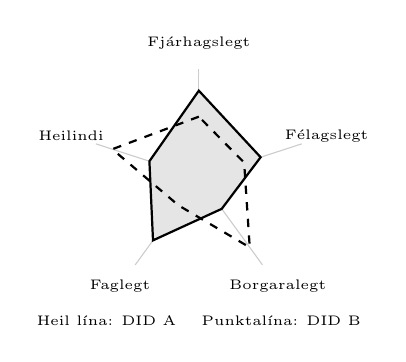
\begin{tikzpicture}[scale=0.55]
\foreach \a/\l in {90/Fjárhagslegt,162/Heilindi,234/Faglegt,306/Borgaralegt,18/Félagslegt} {
  \draw[gray!40] (0,0) -- (\a:2.5);
  \node[font=\tiny, align=center] at (\a:3.1) {\l};
  \foreach \r in {0.8,1.6,2.4} {
    \fill[black!15] (\a:\r) circle (0.5pt);
  }
}
\draw[thick, fill=black!10] (90:2.0) -- (162:1.2) -- (234:1.8) -- (306:0.9) -- (18:1.5) -- cycle;
\draw[thick, dashed] (90:1.4) -- (162:2.1) -- (234:0.8) -- (306:2.0) -- (18:1.1) -- cycle;
\node[font=\tiny] at (0,-3.3) {Heil lína: DID A \quad Punktalína: DID B};
\end{tikzpicture}
\caption{Fjölvíddar orðsporsvigrar. Ólík DID sýna ólík snið yfir víddir.}
\label{fig:reputation-radar}
\end{figure}

\subsection{Lýðræðisvætt áhættumat}

RSN lýðræðisvæðir kerfisbundið áhættumat---getu sem nú er samþjöppuð í fjármálastofnunum en á við langt umfram bankastarfsemi. Iðnaðarsamsteypur sem meta áreiðanleika birgja, tryggingafélög sem verðleggja hegðunaráhættu, áreiðanleikakannanir vegna samruna og yfirtaka, mat á líftíma búnaðar í framleiðslu---hvar sem meta þarf áhættu af gagnaðila veitir RSN dreifstýrðan, markaðsdrifinn valkost. Markaður túlkunarþjónusta þýðir hrá fjölvíddar orðsporsgögn yfir í nýtanleg yfirlit og gerir mat á gagnaðila aðgengilegt hverjum þátttakanda gegn jaðarkostnaði.

% ============================================================
% 7. CONSENSUS AND DISPUTE RESOLUTION
% ============================================================
\section{Samstaða og lausn deilna}

\subsection{Líkan dreifstýrðs réttlætis}

RSN endurskilgreinir réttlæti sem tvíhliða samningavandamál. Hótunin um varanlegan, sannreynanlegan orðsporsskaða er áhrifaríkari fæling en dómsmál sem sá skaðaði hefur ekki efni á.

\subsection{Sjálfsprottin samstaða}

Hver þátttakandi viðheldur persónulegum fullnægjuþröskuldi. Heildarsamstaða netsins sprettur fram sem tölfræðilegt meðaltal þúsunda tvíhliða samninga (Mynd~\ref{fig:consensus}). Svar langt yfir samstöðunni (villimannlegt) er dýrt að birta. Svar nálægt samstöðunni (í réttu hlutfalli) er ódýrt. Samstaðan er ekki regla---hún er verðmerki.

\begin{figure}[ht]
\centering
\begin{tikzpicture}[
    person/.style={draw, rounded corners=2pt, minimum width=1.5cm, minimum height=0.5cm, align=center, font=\scriptsize, fill=black!5},
    arr/.style={-{Stealth[length=4pt]}, thick}
]
\node[person] (a) at (-2,0) {Strangur\\(hár)};
\node[person] (b) at (0,0) {Raunsær\\(miðlungs)};
\node[person] (c) at (2,0) {Fyrirgefandi\\(lágur)};
\node[person, fill=black!10, minimum width=3cm] (cons) at (0,-1.2) {Netsamstaða\\= tölfr.\ meðaltal};
\node[person] (exp) at (-2,-2.4) {Villimannlegt\\dýrt};
\node[person, double] (prop) at (0,-2.4) {Í réttu hlutfalli\\ódýrt};
\node[person] (neg) at (2,-2.4) {Vanrækjandi\\dýrt};

\draw[arr] (a) -- (cons);
\draw[arr] (b) -- (cons);
\draw[arr] (c) -- (cons);
\draw[arr] (cons) -- (exp);
\draw[arr] (cons) -- (prop);
\draw[arr] (cons) -- (neg);
\end{tikzpicture}
\caption{Sjálfsprottin samstaða úr einstaklingsbundnum fullnægjuþröskuldum.}
\label{fig:consensus}
\end{figure}

\subsection{Kvörðun refsingar}

Hver DID-handhafi lýsir opinberlega yfir viðbrögðum við tilteknum flokkum misferlis. Óhóflega harðar eða linar yfirlýsingar draga að sér neikvæð orðsporsmerki. Yfirlýsingar í réttu hlutfalli eru samþykktar án núnings---sjálfkvarðandi refsikerfi.

Samstöðuyfirlýsingar sæta sjálfar hræsnisgreiningu: að skuldbinda sig í orði til samstöðuafstöðu en haga sér ósamkvæmt er orðsporsbrot alvarlegra en undirliggjandi frávikið, þar sem það sýnir ásetningsblekkingu.

\subsection{Framsal}

Öll starfsemi innan DID---með einni undantekningu---má framselja til annars DID. \textbf{Viðfangshlutverkið---það DID sem hegðun þess staðhæfingin fjallar um---er ekki hægt að framselja; það er óframseljanlega bundið auðkennishandhafanum sem staðhæfingin vísar til.} Hin virku hlutverkin---Útgefandi, Yfirvald, Vitni, Sannreynandi---má framselja til tilnefnds fulltrúa-DID, hvort sem er til sannreyningar, framlagningar staðhæfinga, samstöðuþátttöku eða lausnar deilna. Framsal er afturkallanlegt hvenær sem er. Þetta gerir kleifa sérhæfingu (t.d. faglega sannreyningarþjónustu) á meðan handhafinn heldur endanlegri stjórn og ábyrgð. Framsal á við um allt kerfið og er ómissandi fyrir skalanleika.

\subsection{Frá einstaklingssiðferði til sjálfsprottins samfélagssáttmála}

Yfirlýst stefna hvers DID er formgerving einstaklingssiðferðis: hvað handhafinn telur viðunandi, hvernig hann bregst við tilteknum hegðunum, hvað hann krefst af gagnaðilum. Þessar stefnur eru ekki lagðar á af kerfishönnuði---þær eru valdar af hverjum þátttakanda og settar fram á vélalæsilegu formi.

Þessi formgerving gerir kleift þriggja stiga tilkomu. Í fyrsta lagi er einstaklingssiðferði kóðað sem \textbf{stefna}---sett yfirlýstra reglna, þröskulda og viðbragðsfalla sem DID skuldbindur sig til að fylgja. Í öðru lagi framleiðir heildarsafn allra stefna um netið \textbf{sjálfsprottið siðferði} (emergent ethics)---tölfræðilega greinanlegar viðmiðanir sem enginn einstakur þátttakandi hannaði en spretta af samspili þúsunda einstaklingsbundinna siðferðilegra afstaðna~\cite{durkheim1893}. Í þriðja lagi mynda þessar sjálfsprottnu siðferðilegu viðmiðanir, settar fram sem sameiginlegar hegðunarviðmiðanir framfylgt um tvíhliða verðmerki, \textbf{mælanlegan samfélagssáttmála}---ekki fræðilega hugsmíð sem enginn undirritaði~\cite{rawls1971}, heldur reynslulega greinanlegt sett reglna undirbyggt raunverulegri hegðun.

Þetta ferli speglar niðurstöður úr kenningunni um siðferðilegar undirstöður~\cite{haidt2012}: mannlegt siðferði er innsæisbundið, fjölhyggjulegt og menningarlega breytilegt. RSN krefst ekki siðferðilegrar samstöðu sem inntaks; það framleiðir hegðunarsamstöðu sem afurð. Sá samfélagssáttmáli sem af þessu leiðir er ekki kyrrstæður---hann þróast eftir því sem þátttakendur bætast við, hverfa á braut og aðlaga stefnur sínar sem svar við endurgjöf netsins. Ólíkt klassískri samfélagssáttmálakenningu er þessi sáttmáli afturkallanlegur, greinanlegur og framfylgjanlegur án fullveldishafa.

% ============================================================
% 8. ECONOMIC MODEL
% ============================================================
\section{Efnahagslíkan}

Fyrri kaflar lýstu verkfæri---sannreyningarþáttum RSN, kostnaðaruppbyggingu og sjálfsprottinni samstöðu. Þessi kafli lýsir aðferðafræði til að beita þessu verkfæri á umskipti í skatt- og stjórnarháttum. Verkfærið er almenns eðlis; aðferðafræðin hér að neðan er ein möguleg beiting.

\subsection{Hvatauppbygging}

Orðspor sem fjármagn skapar beina hvata til heiðarlegrar hegðunar. Í venjulegum rekstri byggja þátttakendur upp orðspor eðlilega með daglegum viðskiptum og uppfylltum skuldbindingum. Meginútgjöldin eru á \emph{neikvæðar} staðhæfingar---að skrá skaða sem aðrir valda. Þessi ósamhverfa hvetur til nytsamlegrar, áreiðanlegrar hegðunar: að vera heiðarlegur kostar ekkert aukalega, á meðan það að vera skaðlegur skapar skjalfesta slóð sem aðrir munu greiða fyrir að varðveita. Hræsni---að lýsa yfir reglum án þess að fylgja þeim---er dýrasta bilunarhamurinn, þar sem hún sýnir ásetningsblekkingu.

\subsection{Samsíða skattkerfi}

Þrír þættir gera samkeppnisþrýsting mögulegan: (1)~\textbf{Einfaldur skattur}---eitt hlutfallslegt gjald án undantekninga, upphaflega lítillega undir núverandi raunhlutfalli; (2)~\textbf{Rafræn skráning útgjalda} (Electronic Spending Registration, ESR)---sem snýr tékkneska EET-líkaninu við svo borgarar hafi eftirlit með útgjöldum ríkisins; (3)~\textbf{Borgarastýrð skattúthlutun}---sem hefst í fáeinum prósentum á fyrsta ári og nær, eftir áratug, hvar sem er frá lágum tveggja stafa tölum upp í fullkomin umskipti yfir í borgarastýrt kerfi, allt eftir hraða upptöku. Raunverulegur hraði er háður því hversu hratt frjálsmarkaðsvalkostir við ríkisþjónustu spretta upp og vilja ríkisins til að vinna með umskiptunum; fall tímans þarf ekki að vera línulegt, og engin ástæða er til að setja efri mörk á hvar upptaka gæti að lokum lent.

% ============================================================
% 9. MIGRATION PATH
% ============================================================
\section{Umskiptaleið}

Umskiptin fara fram í þremur áföngum (Mynd~\ref{fig:migration}): \textbf{Áfangi~1: Yfirlag} (RSN sem upplýsingalag, ríkið eini veitandinn), \textbf{Áfangi~2: Samkeppni} (RSN veitir virka valkosti, tvíkerfisnotkun), og \textbf{Áfangi~3: Umskipti} (RSN skarar fram úr ríkisígildum, sjálfviljug flutningur). Umskiptin eru afturkræf á hverju stigi.

\begin{figure}[ht]
\centering
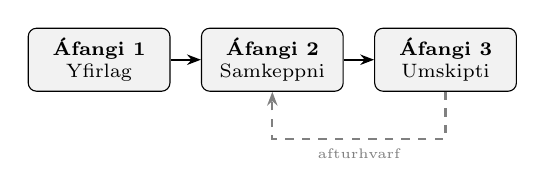
\begin{tikzpicture}[
    phase/.style={draw, rounded corners=3pt, minimum width=1.8cm, minimum height=0.8cm, align=center, font=\scriptsize, fill=black!5},
    arr/.style={-{Stealth[length=5pt]}, thick}
]
\node[phase] (p1) at (0,0) {\textbf{Áfangi 1}\\Yfirlag};
\node[phase] (p2) at (2.2,0) {\textbf{Áfangi 2}\\Samkeppni};
\node[phase] (p3) at (4.4,0) {\textbf{Áfangi 3}\\Umskipti};

\draw[arr] (p1) -- (p2);
\draw[arr] (p2) -- (p3);
\draw[arr, dashed, gray] (p3.south) -- ++(0,-0.6) -| node[below,font=\tiny,pos=0.25] {afturhvarf} (p2.south);
\end{tikzpicture}
\caption{Þriggja áfanga umskipti---afturkræf á hverju stigi.}
\label{fig:migration}
\end{figure}

Meginþrýstiþátturinn er skattalegur: þegar skilyrtir skattgreiðendur ná ,,efnahagslega umtalsverðum minnihluta $X$``---hópi nógu stórum til að kúgun gegn honum valdi ekki-hverfandi efnahagslegu tjóni og borgaraleg óhlýðni verði trúverðug ógn---gengur ríkið til samninga. Til skýringar notum við $X \approx 15\%$ af vergri landsframleiðslu, en raunverulegur þröskuldur er háður hverju hagkerfi fyrir sig.

% ============================================================
% 10. SECURITY ANALYSIS
% ============================================================
\section{Öryggisgreining}

Við íhugum fimm flokka andstæðinga: einstaka illa innrætta aðila, skipulagða hópa, fyrirtækjaandstæðinga, andstæðinga á ríkjastigi og andstæðinga á samskiptareglustigi.

\textbf{Sybil-þol}~\cite{douceur2002}. Að byggja upp orðspor krefst viðvarandi, sannreynanlegra samskipta. Kostnaðurinn við árangursríka Sybil-árás vex línulega með fjölda falskra auðkenna og í öðru veldi með markorðsporsstiginu. Að reka mörg DID samhliða er mögulegt en dýrt með ásetningi---hvert auðkenni verður sjálfstætt að safna orðspori með raunverulegri virkni. Í frjálsum samfélögum fælir þessi kostnaður frá lauslegri misnotkun; í einræðisríkjum verða samsíða DID lifunarverkfæri sem gera kleifa hólfaða andspyrnu, neðanjarðarsamhæfingu og öruggari siglingu um svartamarkað.

\textbf{Vörn gegn leynilegu samráði.} Mynstur gagnkvæmra stuðningsyfirlýsinga meðal lokaðra hópa eru greinanleg með greiningu samfélagsgrafs. Orðspors-samsöfnunarföll afsláttarreikna staðhæfingar frá þétt klösuðum upprunum.

\textbf{Andstæðingur á ríkjastigi.} Laukbeining, fjarvera miðstýrðra innviða og dreifing sannreynandahlutverksins um þátttakendagrunninn tryggja að kúgun krefst aðgerða úr öllu hófi við hvaða ávinning sem er.

\textbf{Friðhelgi á móti ábyrgð.} Gervinafnleynd---millistig milli nafnleyndar og auðkennisupplýsinga---gerir DID kleift að safna merkingarbæru orðspori án þess að opinbera raunverulegt auðkenni handhafans.

% ============================================================
% 11. PRIVACY
% ============================================================
\section{Friðhelgisatriði}

Friðhelgislíkan RSN er byggt á gervinafnleynd. Handhafinn stýrir upplýsingagjöf auðkennis: lágmarks (hreint gervinafn), valkvæð (tiltekin skilríki tengd), eða full (löglegt auðkenni tengt). Birtar staðhæfingar eru varanlegar---kerfið styður samhengislega leiðréttingu en ekki eyðingu. Handhafi má yfirgefa málamiðlað DID og byrja upp á nýtt, og afsala sér uppsöfnuðu orðspori.

% ============================================================
% 12. RELATED WORK
% ============================================================
\section{Skyld verk}

W3C DID Core forskriftin~\cite{did2022} og Ceramic Network~\cite{ceramic2023} veita auðkennisgrunninn. EigenTrust~\cite{kamvar2003} sýndi dreifða orðspors-samsöfnun án miðlægs yfirvalds. SBT~\cite{weyl2022} innleiddu óframseljanleg samfélagstákn. RSN er frábrugðið í áherslu sinni á efnahagslegan kostnað sem gæðasíu og fyrirkomulagi sínu til að verðleggja róttækni.

DAO~\cite{buterin2014} og ferningsleg atkvæðagreiðsla~\cite{buterin2019} sýndu fram á fýsileika dreifstýrðrar stjórnunar. RSN leiðir samstöðu af tvíhliða verðsamningum frekar en atkvæðagreiðslu.

Tillagan byggir á anarkó-kapítalískri kenningu~\cite{rothbard1973,hoppe2001} um einkaþjónustuveitingu en víkur frá henni í tveimur mikilvægum atriðum: hún hannar fyrir hefndargirni og hefndarhvöt frekar en að gera ráð fyrir skynsemi, og hún leggur til smám saman umskipti frekar en byltingu. Hugtakið um sjálfsprottna samfélagssáttmála á sér forvera í kenningu Hayeks um sjálfsprottna skipan~\cite{hayek1973}.

\textbf{Anarkó-agórismi.} RSN deilir umtalsverðum sameiginlegum grunni með agórískri gagnhagfræði~\cite{konkin2006}---sérstaklega áherslunni á að byggja upp samsíða stofnanir og sjálfviljug skipti. Agórismi hefur þó tilhneigingu til að gera ráð fyrir skynsamri eigin hagsmunagæslu sem nægilegri samhæfingaraðferð og skortir oft áþreifanlega umskiptaleið frá núverandi ríkisskipulagi. RSN innlimar með berum orðum ó-skynsamlegar hegðunartilhneigingar og veitir skattalegan þrýstiþátt fyrir smám saman umskipti.

\textbf{Verðleikaræði.} RSN gæti verið fyrsta virka lýsingin á því hvernig verðleikaræði~\cite{young1958} getur sprottið fram sem kerfiseiginleiki frekar en slagorð. Hefðbundin verðleikakerfi bregðast vegna þess að þau krefjast miðlægs yfirvalds til að skilgreina og framfylgja ,,verðleikum``. Í RSN sprettur verðleiki fram af tvíhliða mati: þeir sem skila verðmæti safna orðspori; engin nefnd ákveður hver hefur verðleika.

\textbf{Eign sem forréttindi.} RSN víkur í grundvallaratriðum frá anarkó-kapítalískri og austurríska-skólans meðferð eignaréttar sem náttúrulegs og algilds. Í RSN-rammanum er eign \emph{forréttindi}---samfélagsleg viðurkenning sem, í öfgatilfellum, samfélagið getur afturkallað þegar þátttakandi brýtur í grundvallaratriðum gegn sameiginlegum viðmiðunum (svik, neitun um að verja samfélagið í tilvistarkreppu, kerfisbundin arðrán). Þetta er ekki eignaupptaka ríkisins heldur afturköllun samfélagslegrar viðurkenningar af neti tvíhliða tengsla.

% ============================================================
% 13. LIMITATIONS
% ============================================================
\section{Umræða og takmarkanir}

\textbf{Kaldræsing.} Verðmæti RSN er háð netáhrifum; snemmnotendur standa frammi fyrir takmörkuðu verðmæti þar til þátttaka nær þröskuldi. Samt sem áður, jafnvel frá fyrstu stigum, þjónar DID-netið sem gagnlegur viðbótarupplýsingaruppruni. Búist er við að snemmbúið orðsporsmat og yfirvaldsmat þróist smám saman með aukinni fágun.

\textbf{Sníkjuvörn og aðgangsstýring.} Skotmarks-DID mega leggja stigskipt gjöld og aðgangstakmarkanir á fyrirspurnir frá láorðspora DID. Þetta er ekki tvíundarlegt heldur samfelldur skali: því minna orðspor sem fyrirspyrjandi DID hefur, því minni upplýsingar fær það, því lengur bíður það, og því meira greiðir það. Þetta fyrirkomulag hvetur til raunverulegrar þátttöku umfram óvirkrar neyslu.

\textbf{Ójöfnuður aðgangs.} Kostnaðurinn við að birta staðhæfingar getur síað út lögmætar kvartanir frá efnahagslega illa stæðum þátttakendum. Mildun: sérhver þátttakandi þjónar samtímis sem hugsanlegur sannreynandi (eða framselur það hlutverk) og aflar sannreyningargjalda. Yfir nægilega langt tímabil ætti ó-róttækur þátttakandi að nálgast fjárhagslegt hlutleysi---sannreyningartekjur jafna nokkurn veginn út birtingarkostnað. Þetta er tölfræðileg vænting, ekki trygging.

\textbf{Ójöfnuður orðspors.} Snemmnotendur safna forskoti sem getur skapað hindranir fyrir síðkomna. Orðsporsmat er þó framkvæmt af þriðju-aðila veitendum sem geta valið að milda forskot snemmnotenda með samsöfnunarreikniritum sínum. Að vera fyrstur með gott orðspor er lögmætt hlutfallslegt efnahagslegt forskot---og það er meðvitað hannað.

\textbf{Opnar spurningar.} Ákjósanleg kostnaðarföll, samsöfnunarstaðlar, stjórnun samskiptareglna og samspil við gervigreindarframleidd tilbúin orðsporsgögn eru áfram svið framtíðarvinnu.

Þessi grein heldur því ekki fram að RSN muni framleiða ákjósanlegar niðurstöður við allar aðstæður. Hún heldur því fram að RSN sé \emph{fýsilegur} valkostur---tæknilega útfæranlegur, efnahagslega sjálfbær og samfélagslega samhæfur mannlegum hegðunartilhneigingum eins og þær eru í raun og veru.

% ============================================================
% 14. CONCLUSION
% ============================================================
\section{Niðurstaða}

Þessi grein hefur kynnt orðspors-samfélagsnetið, dreifstýrða samskiptareglu sem gerir kleif gervinafnbundin, sannreynanleg orðsporsskipti. Reglan um dýra róttækni tryggir að svikafullar staðhæfingar eru verðlagðar út án ritskoðunar. Fyrirhuguð umskiptaleið gerir kleif smám saman, afturkræf umskipti frá núverandi stofnunum. Hönnunin innlimar mannlegt eðli eins og það er---þar með talið smásál, hefndargirni og löngun eftir hefndarfullnægju---frekar en að krefjast hugmyndafræðilegrar umbreytingar. Niðurstaðan er ekki útópía heldur kerfi þar sem réttlæti er aðgengilegt, orðspor er áunnið, og kostnaður misferlis er borinn af þeim aðila sem olli því.

% ============================================================
% REFERENCES
% ============================================================
\bibliography{references}

\end{document}
